\documentclass[twoside]{article}

% Packages required by doxygen
\usepackage{fixltx2e}
\usepackage{calc}
\usepackage{doxygen}
\usepackage[export]{adjustbox} % also loads graphicx
\usepackage{graphicx}
\usepackage[utf8]{inputenc}
\usepackage{makeidx}
\usepackage{multicol}
\usepackage{multirow}
\PassOptionsToPackage{warn}{textcomp}
\usepackage{textcomp}
\usepackage[nointegrals]{wasysym}
\usepackage[table]{xcolor}

% Font selection
\usepackage[T1]{fontenc}
\usepackage[scaled=.90]{helvet}
\usepackage{courier}
\usepackage{amssymb}
\usepackage{sectsty}
\renewcommand{\familydefault}{\sfdefault}
\allsectionsfont{%
  \fontseries{bc}\selectfont%
  \color{darkgray}%
}
\renewcommand{\DoxyLabelFont}{%
  \fontseries{bc}\selectfont%
  \color{darkgray}%
}
\newcommand{\+}{\discretionary{\mbox{\scriptsize$\hookleftarrow$}}{}{}}

% Page & text layout
\usepackage{geometry}
\geometry{%
  a4paper,%
  top=2.5cm,%
  bottom=2.5cm,%
  left=2.5cm,%
  right=2.5cm%
}
\tolerance=750
\hfuzz=15pt
\hbadness=750
\setlength{\emergencystretch}{15pt}
\setlength{\parindent}{0cm}
\setlength{\parskip}{3ex plus 2ex minus 2ex}
\makeatletter
\renewcommand{\paragraph}{%
  \@startsection{paragraph}{4}{0ex}{-1.0ex}{1.0ex}{%
    \normalfont\normalsize\bfseries\SS@parafont%
  }%
}
\renewcommand{\subparagraph}{%
  \@startsection{subparagraph}{5}{0ex}{-1.0ex}{1.0ex}{%
    \normalfont\normalsize\bfseries\SS@subparafont%
  }%
}
\makeatother

% Headers & footers
\usepackage{fancyhdr}
\pagestyle{fancyplain}
\fancyhead[LE]{\fancyplain{}{\bfseries\thepage}}
\fancyhead[CE]{\fancyplain{}{}}
\fancyhead[RE]{\fancyplain{}{\bfseries\leftmark}}
\fancyhead[LO]{\fancyplain{}{\bfseries\rightmark}}
\fancyhead[CO]{\fancyplain{}{}}
\fancyhead[RO]{\fancyplain{}{\bfseries\thepage}}
\fancyfoot[LE]{\fancyplain{}{}}
\fancyfoot[CE]{\fancyplain{}{}}
\fancyfoot[RE]{\fancyplain{}{\bfseries\scriptsize Generated by Doxygen }}
\fancyfoot[LO]{\fancyplain{}{\bfseries\scriptsize Generated by Doxygen }}
\fancyfoot[CO]{\fancyplain{}{}}
\fancyfoot[RO]{\fancyplain{}{}}
\renewcommand{\footrulewidth}{0.4pt}
\renewcommand{\sectionmark}[1]{%
  \markright{\thesection\ #1}%
}

% Indices & bibliography
\usepackage{natbib}
\usepackage[titles]{tocloft}
\setcounter{tocdepth}{3}
\setcounter{secnumdepth}{5}
\makeindex

% Hyperlinks (required, but should be loaded last)
\usepackage{ifpdf}
\ifpdf
  \usepackage[pdftex,pagebackref=true]{hyperref}
\else
  \usepackage[ps2pdf,pagebackref=true]{hyperref}
\fi
\hypersetup{%
  colorlinks=true,%
  linkcolor=blue,%
  citecolor=blue,%
  unicode%
}

% Custom commands
\newcommand{\clearemptydoublepage}{%
  \newpage{\pagestyle{empty}\cleardoublepage}%
}

\usepackage{caption}
\captionsetup{labelsep=space,justification=centering,font={bf},singlelinecheck=off,skip=4pt,position=top}

%===== C O N T E N T S =====

\begin{document}

% Titlepage & ToC
\hypersetup{pageanchor=false,
             bookmarksnumbered=true,
             pdfencoding=unicode
            }
\pagenumbering{roman}
\begin{titlepage}
\vspace*{7cm}
\begin{center}%
{\Large Ilda Reader \\[1ex]\large 1.\+0 }\\
\vspace*{1cm}
{\large Generated by Doxygen 1.8.11}\\
\end{center}
\end{titlepage}
\tableofcontents
\pagenumbering{arabic}
\hypersetup{pageanchor=true}

%--- Begin generated contents ---
\section{Data Structure Index}
\subsection{Data Structures}
Here are the data structures with brief descriptions\+:\begin{DoxyCompactList}
\item\contentsline{section}{\hyperlink{structheader__ilda}{header\+\_\+ilda} \\*Data structure which contains the ilda header fields }{\pageref{structheader__ilda}}{}
\item\contentsline{section}{\hyperlink{structpalette}{palette} \\*Format 2, colour palette for the formats using colour index }{\pageref{structpalette}}{}
\item\contentsline{section}{\hyperlink{structpoint2__d}{point2\+\_\+d} \\*Format 1, size of 6 bytes. 2D point with colour index }{\pageref{structpoint2__d}}{}
\item\contentsline{section}{\hyperlink{structpoint2__d__true}{point2\+\_\+d\+\_\+true} \\*Format 5, size of 8 bytes. 2D point with true colour structure }{\pageref{structpoint2__d__true}}{}
\item\contentsline{section}{\hyperlink{structpoint3__d}{point3\+\_\+d} \\*Format 0, size of 8 bytes. 3D point with colour index }{\pageref{structpoint3__d}}{}
\item\contentsline{section}{\hyperlink{structpoint3__d__true}{point3\+\_\+d\+\_\+true} \\*Format 4, size of 10 bytes. 3D point with true colour structure }{\pageref{structpoint3__d__true}}{}
\item\contentsline{section}{\hyperlink{structtrue__color}{true\+\_\+color} \\*Colour data structure for the true colour formats }{\pageref{structtrue__color}}{}
\end{DoxyCompactList}

\section{File Index}
\subsection{File List}
Here is a list of all files with brief descriptions\+:\begin{DoxyCompactList}
\item\contentsline{section}{\hyperlink{ilda__reader_8c}{ilda\+\_\+reader.\+c} }{\pageref{ilda__reader_8c}}{}
\item\contentsline{section}{\hyperlink{ilda__reader_8h}{ilda\+\_\+reader.\+h} }{\pageref{ilda__reader_8h}}{}
\item\contentsline{section}{\hyperlink{main_8c}{main.\+c} }{\pageref{main_8c}}{}
\end{DoxyCompactList}

\section{Data Structure Documentation}
\hypertarget{structheader__ilda}{}\subsection{header\+\_\+ilda Struct Reference}
\label{structheader__ilda}\index{header\+\_\+ilda@{header\+\_\+ilda}}


Data structure which contains the ilda header fields.  




{\ttfamily \#include $<$ilda\+\_\+reader.\+h$>$}

\subsubsection*{Data Fields}
\begin{DoxyCompactItemize}
\item 
char \hyperlink{structheader__ilda_acab5c5e13a661c741491e3d391d2895c}{ilda} \mbox{[}4\mbox{]}
\item 
\hyperlink{ilda__reader_8h_a0c8186d9b9b7880309c27230bbb5e69d}{byte} \hyperlink{structheader__ilda_aaae9f2afe306fb813729a3a510ff4391}{format\+\_\+code}
\item 
char \hyperlink{structheader__ilda_aac9be6f21d28d900a135e2ef2b69021a}{frame\+\_\+name} \mbox{[}9\mbox{]}
\item 
char \hyperlink{structheader__ilda_ab06e9f2a7b6bf9c58179cbf4e7b23a9a}{company\+\_\+name} \mbox{[}9\mbox{]}
\item 
uint16\+\_\+t \hyperlink{structheader__ilda_a95729a0fc0b7cee4780df158f79e991a}{number\+\_\+of\+\_\+records}
\item 
uint16\+\_\+t \hyperlink{structheader__ilda_a723dc14dfda0468bbc2e4fbdac656a08}{frame\+\_\+number}
\item 
uint16\+\_\+t \hyperlink{structheader__ilda_abdbd29a4c96f05535a9bd17e501089d1}{total\+\_\+frames}
\item 
\hyperlink{ilda__reader_8h_a0c8186d9b9b7880309c27230bbb5e69d}{byte} \hyperlink{structheader__ilda_ae3658833789ef3584a0c059680426d00}{proj\+\_\+number}
\end{DoxyCompactItemize}


\subsubsection{Detailed Description}
Data structure which contains the ilda header fields. 

\subsubsection{Field Documentation}
\index{header\+\_\+ilda@{header\+\_\+ilda}!company\+\_\+name@{company\+\_\+name}}
\index{company\+\_\+name@{company\+\_\+name}!header\+\_\+ilda@{header\+\_\+ilda}}
\paragraph[{\texorpdfstring{company\+\_\+name}{company_name}}]{\setlength{\rightskip}{0pt plus 5cm}char header\+\_\+ilda\+::company\+\_\+name\mbox{[}9\mbox{]}}\hypertarget{structheader__ilda_ab06e9f2a7b6bf9c58179cbf4e7b23a9a}{}\label{structheader__ilda_ab06e9f2a7b6bf9c58179cbf4e7b23a9a}
\index{header\+\_\+ilda@{header\+\_\+ilda}!format\+\_\+code@{format\+\_\+code}}
\index{format\+\_\+code@{format\+\_\+code}!header\+\_\+ilda@{header\+\_\+ilda}}
\paragraph[{\texorpdfstring{format\+\_\+code}{format_code}}]{\setlength{\rightskip}{0pt plus 5cm}{\bf byte} header\+\_\+ilda\+::format\+\_\+code}\hypertarget{structheader__ilda_aaae9f2afe306fb813729a3a510ff4391}{}\label{structheader__ilda_aaae9f2afe306fb813729a3a510ff4391}
\index{header\+\_\+ilda@{header\+\_\+ilda}!frame\+\_\+name@{frame\+\_\+name}}
\index{frame\+\_\+name@{frame\+\_\+name}!header\+\_\+ilda@{header\+\_\+ilda}}
\paragraph[{\texorpdfstring{frame\+\_\+name}{frame_name}}]{\setlength{\rightskip}{0pt plus 5cm}char header\+\_\+ilda\+::frame\+\_\+name\mbox{[}9\mbox{]}}\hypertarget{structheader__ilda_aac9be6f21d28d900a135e2ef2b69021a}{}\label{structheader__ilda_aac9be6f21d28d900a135e2ef2b69021a}
\index{header\+\_\+ilda@{header\+\_\+ilda}!frame\+\_\+number@{frame\+\_\+number}}
\index{frame\+\_\+number@{frame\+\_\+number}!header\+\_\+ilda@{header\+\_\+ilda}}
\paragraph[{\texorpdfstring{frame\+\_\+number}{frame_number}}]{\setlength{\rightskip}{0pt plus 5cm}uint16\+\_\+t header\+\_\+ilda\+::frame\+\_\+number}\hypertarget{structheader__ilda_a723dc14dfda0468bbc2e4fbdac656a08}{}\label{structheader__ilda_a723dc14dfda0468bbc2e4fbdac656a08}
\index{header\+\_\+ilda@{header\+\_\+ilda}!ilda@{ilda}}
\index{ilda@{ilda}!header\+\_\+ilda@{header\+\_\+ilda}}
\paragraph[{\texorpdfstring{ilda}{ilda}}]{\setlength{\rightskip}{0pt plus 5cm}char header\+\_\+ilda\+::ilda\mbox{[}4\mbox{]}}\hypertarget{structheader__ilda_acab5c5e13a661c741491e3d391d2895c}{}\label{structheader__ilda_acab5c5e13a661c741491e3d391d2895c}
\index{header\+\_\+ilda@{header\+\_\+ilda}!number\+\_\+of\+\_\+records@{number\+\_\+of\+\_\+records}}
\index{number\+\_\+of\+\_\+records@{number\+\_\+of\+\_\+records}!header\+\_\+ilda@{header\+\_\+ilda}}
\paragraph[{\texorpdfstring{number\+\_\+of\+\_\+records}{number_of_records}}]{\setlength{\rightskip}{0pt plus 5cm}uint16\+\_\+t header\+\_\+ilda\+::number\+\_\+of\+\_\+records}\hypertarget{structheader__ilda_a95729a0fc0b7cee4780df158f79e991a}{}\label{structheader__ilda_a95729a0fc0b7cee4780df158f79e991a}
\index{header\+\_\+ilda@{header\+\_\+ilda}!proj\+\_\+number@{proj\+\_\+number}}
\index{proj\+\_\+number@{proj\+\_\+number}!header\+\_\+ilda@{header\+\_\+ilda}}
\paragraph[{\texorpdfstring{proj\+\_\+number}{proj_number}}]{\setlength{\rightskip}{0pt plus 5cm}{\bf byte} header\+\_\+ilda\+::proj\+\_\+number}\hypertarget{structheader__ilda_ae3658833789ef3584a0c059680426d00}{}\label{structheader__ilda_ae3658833789ef3584a0c059680426d00}
\index{header\+\_\+ilda@{header\+\_\+ilda}!total\+\_\+frames@{total\+\_\+frames}}
\index{total\+\_\+frames@{total\+\_\+frames}!header\+\_\+ilda@{header\+\_\+ilda}}
\paragraph[{\texorpdfstring{total\+\_\+frames}{total_frames}}]{\setlength{\rightskip}{0pt plus 5cm}uint16\+\_\+t header\+\_\+ilda\+::total\+\_\+frames}\hypertarget{structheader__ilda_abdbd29a4c96f05535a9bd17e501089d1}{}\label{structheader__ilda_abdbd29a4c96f05535a9bd17e501089d1}


The documentation for this struct was generated from the following file\+:\begin{DoxyCompactItemize}
\item 
\hyperlink{ilda__reader_8h}{ilda\+\_\+reader.\+h}\end{DoxyCompactItemize}

\hypertarget{structpalette}{}\subsection{palette Struct Reference}
\label{structpalette}\index{palette@{palette}}


format 2, colour palette for the formats using colour index  




{\ttfamily \#include $<$ilda\+\_\+reader.\+h$>$}

\subsubsection*{Data Fields}
\begin{DoxyCompactItemize}
\item 
\hyperlink{ilda__reader_8h_a0c8186d9b9b7880309c27230bbb5e69d}{byte} \hyperlink{structpalette_af572ea74d0b7cae592894591ec7c2d00}{blue}
\item 
\hyperlink{ilda__reader_8h_a0c8186d9b9b7880309c27230bbb5e69d}{byte} \hyperlink{structpalette_a5063d35ce5e5623bc9bdfc75280f800b}{green}
\item 
\hyperlink{ilda__reader_8h_a0c8186d9b9b7880309c27230bbb5e69d}{byte} \hyperlink{structpalette_a4ddb05dff589a890711966e7774e75d2}{red}
\end{DoxyCompactItemize}


\subsubsection{Detailed Description}
format 2, colour palette for the formats using colour index 

\subsubsection{Field Documentation}
\index{palette@{palette}!blue@{blue}}
\index{blue@{blue}!palette@{palette}}
\paragraph[{\texorpdfstring{blue}{blue}}]{\setlength{\rightskip}{0pt plus 5cm}{\bf byte} palette\+::blue}\hypertarget{structpalette_af572ea74d0b7cae592894591ec7c2d00}{}\label{structpalette_af572ea74d0b7cae592894591ec7c2d00}
\index{palette@{palette}!green@{green}}
\index{green@{green}!palette@{palette}}
\paragraph[{\texorpdfstring{green}{green}}]{\setlength{\rightskip}{0pt plus 5cm}{\bf byte} palette\+::green}\hypertarget{structpalette_a5063d35ce5e5623bc9bdfc75280f800b}{}\label{structpalette_a5063d35ce5e5623bc9bdfc75280f800b}
\index{palette@{palette}!red@{red}}
\index{red@{red}!palette@{palette}}
\paragraph[{\texorpdfstring{red}{red}}]{\setlength{\rightskip}{0pt plus 5cm}{\bf byte} palette\+::red}\hypertarget{structpalette_a4ddb05dff589a890711966e7774e75d2}{}\label{structpalette_a4ddb05dff589a890711966e7774e75d2}


The documentation for this struct was generated from the following file\+:\begin{DoxyCompactItemize}
\item 
\hyperlink{ilda__reader_8h}{ilda\+\_\+reader.\+h}\end{DoxyCompactItemize}

\hypertarget{structpoint2__d}{}\subsection{point2\+\_\+d Struct Reference}
\label{structpoint2__d}\index{point2\+\_\+d@{point2\+\_\+d}}


format 1, size of 6 bytes. 2D point with colour index  




{\ttfamily \#include $<$ilda\+\_\+reader.\+h$>$}

\subsubsection*{Data Fields}
\begin{DoxyCompactItemize}
\item 
int16\+\_\+t \hyperlink{structpoint2__d_ace7ebdd2a9d9558104cbddcaf0cbd1ba}{x\+\_\+coord}
\item 
int16\+\_\+t \hyperlink{structpoint2__d_aee96b403bc3c20867009b8fcddac3399}{y\+\_\+coord}
\item 
\hyperlink{ilda__reader_8h_a0c8186d9b9b7880309c27230bbb5e69d}{byte} \hyperlink{structpoint2__d_ac4b500addb03876aad385716669899fd}{status\+\_\+code}
\item 
\hyperlink{ilda__reader_8h_a0c8186d9b9b7880309c27230bbb5e69d}{byte} \hyperlink{structpoint2__d_ac31c9a95ce5930655ad1de27d18bec2d}{color\+\_\+index}
\end{DoxyCompactItemize}


\subsubsection{Detailed Description}
format 1, size of 6 bytes. 2D point with colour index 

\subsubsection{Field Documentation}
\index{point2\+\_\+d@{point2\+\_\+d}!color\+\_\+index@{color\+\_\+index}}
\index{color\+\_\+index@{color\+\_\+index}!point2\+\_\+d@{point2\+\_\+d}}
\paragraph[{\texorpdfstring{color\+\_\+index}{color_index}}]{\setlength{\rightskip}{0pt plus 5cm}{\bf byte} point2\+\_\+d\+::color\+\_\+index}\hypertarget{structpoint2__d_ac31c9a95ce5930655ad1de27d18bec2d}{}\label{structpoint2__d_ac31c9a95ce5930655ad1de27d18bec2d}
\index{point2\+\_\+d@{point2\+\_\+d}!status\+\_\+code@{status\+\_\+code}}
\index{status\+\_\+code@{status\+\_\+code}!point2\+\_\+d@{point2\+\_\+d}}
\paragraph[{\texorpdfstring{status\+\_\+code}{status_code}}]{\setlength{\rightskip}{0pt plus 5cm}{\bf byte} point2\+\_\+d\+::status\+\_\+code}\hypertarget{structpoint2__d_ac4b500addb03876aad385716669899fd}{}\label{structpoint2__d_ac4b500addb03876aad385716669899fd}
\index{point2\+\_\+d@{point2\+\_\+d}!x\+\_\+coord@{x\+\_\+coord}}
\index{x\+\_\+coord@{x\+\_\+coord}!point2\+\_\+d@{point2\+\_\+d}}
\paragraph[{\texorpdfstring{x\+\_\+coord}{x_coord}}]{\setlength{\rightskip}{0pt plus 5cm}int16\+\_\+t point2\+\_\+d\+::x\+\_\+coord}\hypertarget{structpoint2__d_ace7ebdd2a9d9558104cbddcaf0cbd1ba}{}\label{structpoint2__d_ace7ebdd2a9d9558104cbddcaf0cbd1ba}
\index{point2\+\_\+d@{point2\+\_\+d}!y\+\_\+coord@{y\+\_\+coord}}
\index{y\+\_\+coord@{y\+\_\+coord}!point2\+\_\+d@{point2\+\_\+d}}
\paragraph[{\texorpdfstring{y\+\_\+coord}{y_coord}}]{\setlength{\rightskip}{0pt plus 5cm}int16\+\_\+t point2\+\_\+d\+::y\+\_\+coord}\hypertarget{structpoint2__d_aee96b403bc3c20867009b8fcddac3399}{}\label{structpoint2__d_aee96b403bc3c20867009b8fcddac3399}


The documentation for this struct was generated from the following file\+:\begin{DoxyCompactItemize}
\item 
\hyperlink{ilda__reader_8h}{ilda\+\_\+reader.\+h}\end{DoxyCompactItemize}

\hypertarget{structpoint2__d__true}{}\subsection{point2\+\_\+d\+\_\+true Struct Reference}
\label{structpoint2__d__true}\index{point2\+\_\+d\+\_\+true@{point2\+\_\+d\+\_\+true}}


format 5, size of 8 bytes. 2D point with true colour structure  




{\ttfamily \#include $<$ilda\+\_\+reader.\+h$>$}



Collaboration diagram for point2\+\_\+d\+\_\+true\+:\nopagebreak
\begin{figure}[H]
\begin{center}
\leavevmode
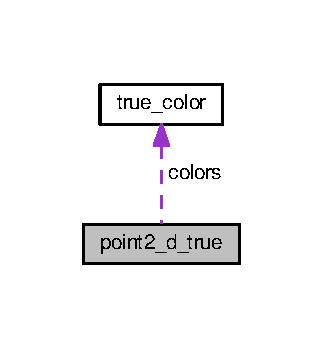
\includegraphics[width=155pt]{structpoint2__d__true__coll__graph}
\end{center}
\end{figure}
\subsubsection*{Data Fields}
\begin{DoxyCompactItemize}
\item 
int16\+\_\+t \hyperlink{structpoint2__d__true_a7625206de81434de8e73402879ef4097}{x\+\_\+coord}
\item 
int16\+\_\+t \hyperlink{structpoint2__d__true_a60cba7c6a2b3a2484708a1f4b89cae3b}{y\+\_\+coord}
\item 
\hyperlink{ilda__reader_8h_a0c8186d9b9b7880309c27230bbb5e69d}{byte} \hyperlink{structpoint2__d__true_adf21432adfbce8fbec69ae4032f0efdd}{status\+\_\+code}
\item 
struct \hyperlink{structtrue__color}{true\+\_\+color} \hyperlink{structpoint2__d__true_a9d3523137b35d48f7c1999de020bb3ed}{colors}
\end{DoxyCompactItemize}


\subsubsection{Detailed Description}
format 5, size of 8 bytes. 2D point with true colour structure 

\subsubsection{Field Documentation}
\index{point2\+\_\+d\+\_\+true@{point2\+\_\+d\+\_\+true}!colors@{colors}}
\index{colors@{colors}!point2\+\_\+d\+\_\+true@{point2\+\_\+d\+\_\+true}}
\paragraph[{\texorpdfstring{colors}{colors}}]{\setlength{\rightskip}{0pt plus 5cm}struct {\bf true\+\_\+color} point2\+\_\+d\+\_\+true\+::colors}\hypertarget{structpoint2__d__true_a9d3523137b35d48f7c1999de020bb3ed}{}\label{structpoint2__d__true_a9d3523137b35d48f7c1999de020bb3ed}
\index{point2\+\_\+d\+\_\+true@{point2\+\_\+d\+\_\+true}!status\+\_\+code@{status\+\_\+code}}
\index{status\+\_\+code@{status\+\_\+code}!point2\+\_\+d\+\_\+true@{point2\+\_\+d\+\_\+true}}
\paragraph[{\texorpdfstring{status\+\_\+code}{status_code}}]{\setlength{\rightskip}{0pt plus 5cm}{\bf byte} point2\+\_\+d\+\_\+true\+::status\+\_\+code}\hypertarget{structpoint2__d__true_adf21432adfbce8fbec69ae4032f0efdd}{}\label{structpoint2__d__true_adf21432adfbce8fbec69ae4032f0efdd}
\index{point2\+\_\+d\+\_\+true@{point2\+\_\+d\+\_\+true}!x\+\_\+coord@{x\+\_\+coord}}
\index{x\+\_\+coord@{x\+\_\+coord}!point2\+\_\+d\+\_\+true@{point2\+\_\+d\+\_\+true}}
\paragraph[{\texorpdfstring{x\+\_\+coord}{x_coord}}]{\setlength{\rightskip}{0pt plus 5cm}int16\+\_\+t point2\+\_\+d\+\_\+true\+::x\+\_\+coord}\hypertarget{structpoint2__d__true_a7625206de81434de8e73402879ef4097}{}\label{structpoint2__d__true_a7625206de81434de8e73402879ef4097}
\index{point2\+\_\+d\+\_\+true@{point2\+\_\+d\+\_\+true}!y\+\_\+coord@{y\+\_\+coord}}
\index{y\+\_\+coord@{y\+\_\+coord}!point2\+\_\+d\+\_\+true@{point2\+\_\+d\+\_\+true}}
\paragraph[{\texorpdfstring{y\+\_\+coord}{y_coord}}]{\setlength{\rightskip}{0pt plus 5cm}int16\+\_\+t point2\+\_\+d\+\_\+true\+::y\+\_\+coord}\hypertarget{structpoint2__d__true_a60cba7c6a2b3a2484708a1f4b89cae3b}{}\label{structpoint2__d__true_a60cba7c6a2b3a2484708a1f4b89cae3b}


The documentation for this struct was generated from the following file\+:\begin{DoxyCompactItemize}
\item 
\hyperlink{ilda__reader_8h}{ilda\+\_\+reader.\+h}\end{DoxyCompactItemize}

\hypertarget{structpoint3__d}{}\subsection{point3\+\_\+d Struct Reference}
\label{structpoint3__d}\index{point3\+\_\+d@{point3\+\_\+d}}


format 0, size of 8 bytes. 3D point with colour index  




{\ttfamily \#include $<$ilda\+\_\+reader.\+h$>$}

\subsubsection*{Data Fields}
\begin{DoxyCompactItemize}
\item 
int16\+\_\+t \hyperlink{structpoint3__d_a82eab6ff9df48322e3252c6556db05e3}{x\+\_\+coord}
\item 
int16\+\_\+t \hyperlink{structpoint3__d_a1ccb895cc6619f81c02aec641282ebcb}{y\+\_\+coord}
\item 
int16\+\_\+t \hyperlink{structpoint3__d_acf2babaff2830180190d111c8958f6af}{z\+\_\+coord}
\item 
\hyperlink{ilda__reader_8h_a0c8186d9b9b7880309c27230bbb5e69d}{byte} \hyperlink{structpoint3__d_ac46953a940fbb65ffed780bcb5ac2ecc}{status\+\_\+code}
\item 
\hyperlink{ilda__reader_8h_a0c8186d9b9b7880309c27230bbb5e69d}{byte} \hyperlink{structpoint3__d_a4db0c777246f6ac7f4d0fc72111e947b}{color\+\_\+index}
\end{DoxyCompactItemize}


\subsubsection{Detailed Description}
format 0, size of 8 bytes. 3D point with colour index 

\subsubsection{Field Documentation}
\index{point3\+\_\+d@{point3\+\_\+d}!color\+\_\+index@{color\+\_\+index}}
\index{color\+\_\+index@{color\+\_\+index}!point3\+\_\+d@{point3\+\_\+d}}
\paragraph[{\texorpdfstring{color\+\_\+index}{color_index}}]{\setlength{\rightskip}{0pt plus 5cm}{\bf byte} point3\+\_\+d\+::color\+\_\+index}\hypertarget{structpoint3__d_a4db0c777246f6ac7f4d0fc72111e947b}{}\label{structpoint3__d_a4db0c777246f6ac7f4d0fc72111e947b}
\index{point3\+\_\+d@{point3\+\_\+d}!status\+\_\+code@{status\+\_\+code}}
\index{status\+\_\+code@{status\+\_\+code}!point3\+\_\+d@{point3\+\_\+d}}
\paragraph[{\texorpdfstring{status\+\_\+code}{status_code}}]{\setlength{\rightskip}{0pt plus 5cm}{\bf byte} point3\+\_\+d\+::status\+\_\+code}\hypertarget{structpoint3__d_ac46953a940fbb65ffed780bcb5ac2ecc}{}\label{structpoint3__d_ac46953a940fbb65ffed780bcb5ac2ecc}
\index{point3\+\_\+d@{point3\+\_\+d}!x\+\_\+coord@{x\+\_\+coord}}
\index{x\+\_\+coord@{x\+\_\+coord}!point3\+\_\+d@{point3\+\_\+d}}
\paragraph[{\texorpdfstring{x\+\_\+coord}{x_coord}}]{\setlength{\rightskip}{0pt plus 5cm}int16\+\_\+t point3\+\_\+d\+::x\+\_\+coord}\hypertarget{structpoint3__d_a82eab6ff9df48322e3252c6556db05e3}{}\label{structpoint3__d_a82eab6ff9df48322e3252c6556db05e3}
\index{point3\+\_\+d@{point3\+\_\+d}!y\+\_\+coord@{y\+\_\+coord}}
\index{y\+\_\+coord@{y\+\_\+coord}!point3\+\_\+d@{point3\+\_\+d}}
\paragraph[{\texorpdfstring{y\+\_\+coord}{y_coord}}]{\setlength{\rightskip}{0pt plus 5cm}int16\+\_\+t point3\+\_\+d\+::y\+\_\+coord}\hypertarget{structpoint3__d_a1ccb895cc6619f81c02aec641282ebcb}{}\label{structpoint3__d_a1ccb895cc6619f81c02aec641282ebcb}
\index{point3\+\_\+d@{point3\+\_\+d}!z\+\_\+coord@{z\+\_\+coord}}
\index{z\+\_\+coord@{z\+\_\+coord}!point3\+\_\+d@{point3\+\_\+d}}
\paragraph[{\texorpdfstring{z\+\_\+coord}{z_coord}}]{\setlength{\rightskip}{0pt plus 5cm}int16\+\_\+t point3\+\_\+d\+::z\+\_\+coord}\hypertarget{structpoint3__d_acf2babaff2830180190d111c8958f6af}{}\label{structpoint3__d_acf2babaff2830180190d111c8958f6af}


The documentation for this struct was generated from the following file\+:\begin{DoxyCompactItemize}
\item 
\hyperlink{ilda__reader_8h}{ilda\+\_\+reader.\+h}\end{DoxyCompactItemize}

\hypertarget{structpoint3__d__true}{}\subsection{point3\+\_\+d\+\_\+true Struct Reference}
\label{structpoint3__d__true}\index{point3\+\_\+d\+\_\+true@{point3\+\_\+d\+\_\+true}}


format 4, size of 10 bytes. 3D point with true colour structure.  




{\ttfamily \#include $<$ilda\+\_\+reader.\+h$>$}



Collaboration diagram for point3\+\_\+d\+\_\+true\+:\nopagebreak
\begin{figure}[H]
\begin{center}
\leavevmode
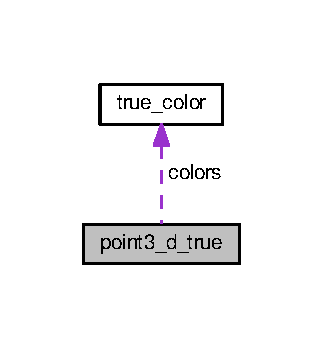
\includegraphics[width=155pt]{structpoint3__d__true__coll__graph}
\end{center}
\end{figure}
\subsubsection*{Data Fields}
\begin{DoxyCompactItemize}
\item 
int16\+\_\+t \hyperlink{structpoint3__d__true_ae2fecb3111aaa9450526d3a8ac54cc2f}{x\+\_\+coord}
\item 
int16\+\_\+t \hyperlink{structpoint3__d__true_a3e9e88bc5533d72da6811340ce578f67}{y\+\_\+coord}
\item 
int16\+\_\+t \hyperlink{structpoint3__d__true_aad4fd09f85d4f8c7d7aa1bf80f7fc7c3}{z\+\_\+coord}
\item 
\hyperlink{ilda__reader_8h_a0c8186d9b9b7880309c27230bbb5e69d}{byte} \hyperlink{structpoint3__d__true_a05766432b1037ce6ddb34874df3245d7}{status\+\_\+code}
\item 
struct \hyperlink{structtrue__color}{true\+\_\+color} \hyperlink{structpoint3__d__true_a439d36e90be604aea553da6d944c4173}{colors}
\end{DoxyCompactItemize}


\subsubsection{Detailed Description}
format 4, size of 10 bytes. 3D point with true colour structure. 

\subsubsection{Field Documentation}
\index{point3\+\_\+d\+\_\+true@{point3\+\_\+d\+\_\+true}!colors@{colors}}
\index{colors@{colors}!point3\+\_\+d\+\_\+true@{point3\+\_\+d\+\_\+true}}
\paragraph[{\texorpdfstring{colors}{colors}}]{\setlength{\rightskip}{0pt plus 5cm}struct {\bf true\+\_\+color} point3\+\_\+d\+\_\+true\+::colors}\hypertarget{structpoint3__d__true_a439d36e90be604aea553da6d944c4173}{}\label{structpoint3__d__true_a439d36e90be604aea553da6d944c4173}
\index{point3\+\_\+d\+\_\+true@{point3\+\_\+d\+\_\+true}!status\+\_\+code@{status\+\_\+code}}
\index{status\+\_\+code@{status\+\_\+code}!point3\+\_\+d\+\_\+true@{point3\+\_\+d\+\_\+true}}
\paragraph[{\texorpdfstring{status\+\_\+code}{status_code}}]{\setlength{\rightskip}{0pt plus 5cm}{\bf byte} point3\+\_\+d\+\_\+true\+::status\+\_\+code}\hypertarget{structpoint3__d__true_a05766432b1037ce6ddb34874df3245d7}{}\label{structpoint3__d__true_a05766432b1037ce6ddb34874df3245d7}
\index{point3\+\_\+d\+\_\+true@{point3\+\_\+d\+\_\+true}!x\+\_\+coord@{x\+\_\+coord}}
\index{x\+\_\+coord@{x\+\_\+coord}!point3\+\_\+d\+\_\+true@{point3\+\_\+d\+\_\+true}}
\paragraph[{\texorpdfstring{x\+\_\+coord}{x_coord}}]{\setlength{\rightskip}{0pt plus 5cm}int16\+\_\+t point3\+\_\+d\+\_\+true\+::x\+\_\+coord}\hypertarget{structpoint3__d__true_ae2fecb3111aaa9450526d3a8ac54cc2f}{}\label{structpoint3__d__true_ae2fecb3111aaa9450526d3a8ac54cc2f}
\index{point3\+\_\+d\+\_\+true@{point3\+\_\+d\+\_\+true}!y\+\_\+coord@{y\+\_\+coord}}
\index{y\+\_\+coord@{y\+\_\+coord}!point3\+\_\+d\+\_\+true@{point3\+\_\+d\+\_\+true}}
\paragraph[{\texorpdfstring{y\+\_\+coord}{y_coord}}]{\setlength{\rightskip}{0pt plus 5cm}int16\+\_\+t point3\+\_\+d\+\_\+true\+::y\+\_\+coord}\hypertarget{structpoint3__d__true_a3e9e88bc5533d72da6811340ce578f67}{}\label{structpoint3__d__true_a3e9e88bc5533d72da6811340ce578f67}
\index{point3\+\_\+d\+\_\+true@{point3\+\_\+d\+\_\+true}!z\+\_\+coord@{z\+\_\+coord}}
\index{z\+\_\+coord@{z\+\_\+coord}!point3\+\_\+d\+\_\+true@{point3\+\_\+d\+\_\+true}}
\paragraph[{\texorpdfstring{z\+\_\+coord}{z_coord}}]{\setlength{\rightskip}{0pt plus 5cm}int16\+\_\+t point3\+\_\+d\+\_\+true\+::z\+\_\+coord}\hypertarget{structpoint3__d__true_aad4fd09f85d4f8c7d7aa1bf80f7fc7c3}{}\label{structpoint3__d__true_aad4fd09f85d4f8c7d7aa1bf80f7fc7c3}


The documentation for this struct was generated from the following file\+:\begin{DoxyCompactItemize}
\item 
\hyperlink{ilda__reader_8h}{ilda\+\_\+reader.\+h}\end{DoxyCompactItemize}

\hypertarget{structtrue__color}{}\subsection{true\+\_\+color Struct Reference}
\label{structtrue__color}\index{true\+\_\+color@{true\+\_\+color}}


Colour data structure for the true colour formats.  




{\ttfamily \#include $<$ilda\+\_\+reader.\+h$>$}

\subsubsection*{Data Fields}
\begin{DoxyCompactItemize}
\item 
\hyperlink{ilda__reader_8h_a0c8186d9b9b7880309c27230bbb5e69d}{byte} \hyperlink{structtrue__color_a10495bcfef39ca3c51caac12dd6e3478}{blue}
\item 
\hyperlink{ilda__reader_8h_a0c8186d9b9b7880309c27230bbb5e69d}{byte} \hyperlink{structtrue__color_aab9c7be436a3fa58b597718cfe071d16}{green}
\item 
\hyperlink{ilda__reader_8h_a0c8186d9b9b7880309c27230bbb5e69d}{byte} \hyperlink{structtrue__color_a8840e16b209c4cfaf42737d2ee98d8a0}{red}
\end{DoxyCompactItemize}


\subsubsection{Detailed Description}
Colour data structure for the true colour formats. 

\subsubsection{Field Documentation}
\index{true\+\_\+color@{true\+\_\+color}!blue@{blue}}
\index{blue@{blue}!true\+\_\+color@{true\+\_\+color}}
\paragraph[{\texorpdfstring{blue}{blue}}]{\setlength{\rightskip}{0pt plus 5cm}{\bf byte} true\+\_\+color\+::blue}\hypertarget{structtrue__color_a10495bcfef39ca3c51caac12dd6e3478}{}\label{structtrue__color_a10495bcfef39ca3c51caac12dd6e3478}
\index{true\+\_\+color@{true\+\_\+color}!green@{green}}
\index{green@{green}!true\+\_\+color@{true\+\_\+color}}
\paragraph[{\texorpdfstring{green}{green}}]{\setlength{\rightskip}{0pt plus 5cm}{\bf byte} true\+\_\+color\+::green}\hypertarget{structtrue__color_aab9c7be436a3fa58b597718cfe071d16}{}\label{structtrue__color_aab9c7be436a3fa58b597718cfe071d16}
\index{true\+\_\+color@{true\+\_\+color}!red@{red}}
\index{red@{red}!true\+\_\+color@{true\+\_\+color}}
\paragraph[{\texorpdfstring{red}{red}}]{\setlength{\rightskip}{0pt plus 5cm}{\bf byte} true\+\_\+color\+::red}\hypertarget{structtrue__color_a8840e16b209c4cfaf42737d2ee98d8a0}{}\label{structtrue__color_a8840e16b209c4cfaf42737d2ee98d8a0}


The documentation for this struct was generated from the following file\+:\begin{DoxyCompactItemize}
\item 
\hyperlink{ilda__reader_8h}{ilda\+\_\+reader.\+h}\end{DoxyCompactItemize}

\section{File Documentation}
\hypertarget{ilda__reader_8c}{}\subsection{ilda\+\_\+reader.\+c File Reference}
\label{ilda__reader_8c}\index{ilda\+\_\+reader.\+c@{ilda\+\_\+reader.\+c}}
{\ttfamily \#include \char`\"{}ilda\+\_\+reader.\+h\char`\"{}}\\*
{\ttfamily \#include $<$stdio.\+h$>$}\\*
{\ttfamily \#include $<$string.\+h$>$}\\*
{\ttfamily \#include $<$stdlib.\+h$>$}\\*
Include dependency graph for ilda\+\_\+reader.\+c\+:\nopagebreak
\begin{figure}[H]
\begin{center}
\leavevmode
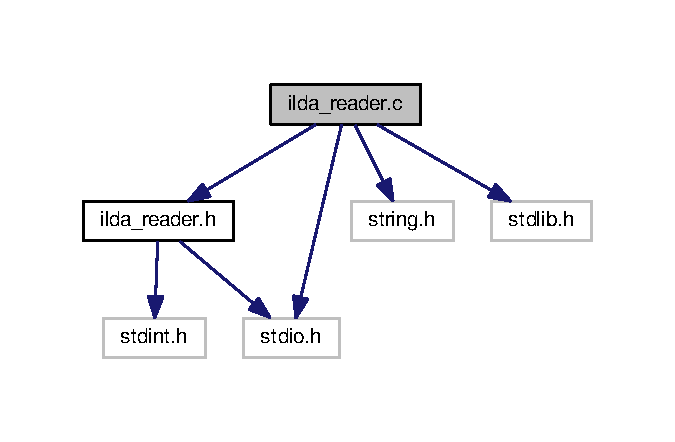
\includegraphics[width=324pt]{ilda__reader_8c__incl}
\end{center}
\end{figure}
\subsubsection*{Macros}
\begin{DoxyCompactItemize}
\item 
\#define \hyperlink{ilda__reader_8c_a8782a401fbf55261460863fc2f8df1ce}{L\+I\+T\+T\+L\+E\+\_\+\+E\+N\+D\+I\+AN}~1
\begin{DoxyCompactList}\small\item\em since the file is in big endian, conversions have to be in place for little endian cpu\textquotesingle{}s \end{DoxyCompactList}\item 
\#define \hyperlink{ilda__reader_8c_a111da81ae5883147168bbb8366377b10}{B}~8$\ast$\hyperlink{ilda__reader_8c_a8782a401fbf55261460863fc2f8df1ce}{L\+I\+T\+T\+L\+E\+\_\+\+E\+N\+D\+I\+AN}
\begin{DoxyCompactList}\small\item\em amount to shift least significant byte, for endianness conversions \end{DoxyCompactList}\item 
\#define \hyperlink{ilda__reader_8c_aa73214aa5f2f94f63d90bb4e3d99fe53}{L}~8$\ast$(!\hyperlink{ilda__reader_8c_a8782a401fbf55261460863fc2f8df1ce}{L\+I\+T\+T\+L\+E\+\_\+\+E\+N\+D\+I\+AN})
\begin{DoxyCompactList}\small\item\em amount to shift most significant byte, for endianness conversions \end{DoxyCompactList}\end{DoxyCompactItemize}
\subsubsection*{Functions}
\begin{DoxyCompactItemize}
\item 
void \hyperlink{ilda__reader_8c_af9fce4ec98c31e5a017b793e5f89a9e0}{print\+\_\+header} (struct \hyperlink{structheader__ilda}{header\+\_\+ilda} hdr)
\item 
int \hyperlink{ilda__reader_8c_acfc7598b101bc5f6551e0eba6079cca5}{read3\+\_\+d} (struct \hyperlink{structpoint3__d}{point3\+\_\+d} $\ast$point, F\+I\+LE $\ast$ins)
\begin{DoxyCompactList}\small\item\em Reads from a file into a \hyperlink{structpoint3__d}{point3\+\_\+d} P\+OD structure, should be called if format code \textquotesingle{}0\textquotesingle{} is encountered. \end{DoxyCompactList}\item 
int \hyperlink{ilda__reader_8c_a6ccfb058e3e717fc6b62a16975aae044}{read2\+\_\+d} (struct \hyperlink{structpoint2__d}{point2\+\_\+d} $\ast$point, F\+I\+LE $\ast$ins)
\begin{DoxyCompactList}\small\item\em Reads from a file into a \hyperlink{structpoint2__d}{point2\+\_\+d} P\+OD structure, should be called if format code \textquotesingle{}1\textquotesingle{} is encountered. \end{DoxyCompactList}\item 
int \hyperlink{ilda__reader_8c_a620cfa9600a541d1c512b0ef7a63b92b}{read\+\_\+palette} (struct \hyperlink{structpalette}{palette} $\ast$point, F\+I\+LE $\ast$ins)
\begin{DoxyCompactList}\small\item\em Reads from a file into a palette P\+OD structure, should be called if format code \textquotesingle{}2\textquotesingle{} is encountered. \end{DoxyCompactList}\item 
int \hyperlink{ilda__reader_8c_ad8543fa23af10e3cdbe44e62c66556a1}{read3\+\_\+dt} (struct \hyperlink{structpoint3__d__true}{point3\+\_\+d\+\_\+true} $\ast$point, F\+I\+LE $\ast$ins)
\begin{DoxyCompactList}\small\item\em Reads from a file into a \hyperlink{structpoint3__d__true}{point3\+\_\+d\+\_\+true} P\+OD structure, should be called if format code \textquotesingle{}4\textquotesingle{} is encountered. \end{DoxyCompactList}\item 
int \hyperlink{ilda__reader_8c_a42c4a3d0ee1c18a464bf952ab9e6e73d}{read2\+\_\+dt} (struct \hyperlink{structpoint2__d__true}{point2\+\_\+d\+\_\+true} $\ast$point, F\+I\+LE $\ast$ins)
\begin{DoxyCompactList}\small\item\em Reads from a file into a \hyperlink{structpoint2__d__true}{point2\+\_\+d\+\_\+true} P\+OD structure, should be called if format code \textquotesingle{}5\textquotesingle{} is encountered. \end{DoxyCompactList}\item 
int \hyperlink{ilda__reader_8c_a658cb1acb17941afee94de570f2197b8}{read\+\_\+ilda\+\_\+header} (struct \hyperlink{structheader__ilda}{header\+\_\+ilda} $\ast$hdr, F\+I\+LE $\ast$ins)
\begin{DoxyCompactList}\small\item\em Puts ilda header information in the {\itshape hdr parameter from the ins} file. \end{DoxyCompactList}\item 
void \hyperlink{ilda__reader_8c_a370b6a4c6d690796ef6e62ff7b2e5f94}{read\+\_\+ilda} ()
\begin{DoxyCompactList}\small\item\em reads the whole ilda file and prints it on the console. Does not buffer anything. Will exit if file is not found. \end{DoxyCompactList}\end{DoxyCompactItemize}


\subsubsection{Macro Definition Documentation}
\index{ilda\+\_\+reader.\+c@{ilda\+\_\+reader.\+c}!B@{B}}
\index{B@{B}!ilda\+\_\+reader.\+c@{ilda\+\_\+reader.\+c}}
\paragraph[{\texorpdfstring{B}{B}}]{\setlength{\rightskip}{0pt plus 5cm}\#define B~8$\ast${\bf L\+I\+T\+T\+L\+E\+\_\+\+E\+N\+D\+I\+AN}}\hypertarget{ilda__reader_8c_a111da81ae5883147168bbb8366377b10}{}\label{ilda__reader_8c_a111da81ae5883147168bbb8366377b10}


amount to shift least significant byte, for endianness conversions 

\index{ilda\+\_\+reader.\+c@{ilda\+\_\+reader.\+c}!L@{L}}
\index{L@{L}!ilda\+\_\+reader.\+c@{ilda\+\_\+reader.\+c}}
\paragraph[{\texorpdfstring{L}{L}}]{\setlength{\rightskip}{0pt plus 5cm}\#define L~8$\ast$(!{\bf L\+I\+T\+T\+L\+E\+\_\+\+E\+N\+D\+I\+AN})}\hypertarget{ilda__reader_8c_aa73214aa5f2f94f63d90bb4e3d99fe53}{}\label{ilda__reader_8c_aa73214aa5f2f94f63d90bb4e3d99fe53}


amount to shift most significant byte, for endianness conversions 

\index{ilda\+\_\+reader.\+c@{ilda\+\_\+reader.\+c}!L\+I\+T\+T\+L\+E\+\_\+\+E\+N\+D\+I\+AN@{L\+I\+T\+T\+L\+E\+\_\+\+E\+N\+D\+I\+AN}}
\index{L\+I\+T\+T\+L\+E\+\_\+\+E\+N\+D\+I\+AN@{L\+I\+T\+T\+L\+E\+\_\+\+E\+N\+D\+I\+AN}!ilda\+\_\+reader.\+c@{ilda\+\_\+reader.\+c}}
\paragraph[{\texorpdfstring{L\+I\+T\+T\+L\+E\+\_\+\+E\+N\+D\+I\+AN}{LITTLE_ENDIAN}}]{\setlength{\rightskip}{0pt plus 5cm}\#define L\+I\+T\+T\+L\+E\+\_\+\+E\+N\+D\+I\+AN~1}\hypertarget{ilda__reader_8c_a8782a401fbf55261460863fc2f8df1ce}{}\label{ilda__reader_8c_a8782a401fbf55261460863fc2f8df1ce}


since the file is in big endian, conversions have to be in place for little endian cpu\textquotesingle{}s 



\subsubsection{Function Documentation}
\index{ilda\+\_\+reader.\+c@{ilda\+\_\+reader.\+c}!print\+\_\+header@{print\+\_\+header}}
\index{print\+\_\+header@{print\+\_\+header}!ilda\+\_\+reader.\+c@{ilda\+\_\+reader.\+c}}
\paragraph[{\texorpdfstring{print\+\_\+header(struct header\+\_\+ilda hdr)}{print_header(struct header_ilda hdr)}}]{\setlength{\rightskip}{0pt plus 5cm}void print\+\_\+header (
\begin{DoxyParamCaption}
\item[{struct {\bf header\+\_\+ilda}}]{hdr}
\end{DoxyParamCaption}
)}\hypertarget{ilda__reader_8c_af9fce4ec98c31e5a017b793e5f89a9e0}{}\label{ilda__reader_8c_af9fce4ec98c31e5a017b793e5f89a9e0}
\index{ilda\+\_\+reader.\+c@{ilda\+\_\+reader.\+c}!read2\+\_\+d@{read2\+\_\+d}}
\index{read2\+\_\+d@{read2\+\_\+d}!ilda\+\_\+reader.\+c@{ilda\+\_\+reader.\+c}}
\paragraph[{\texorpdfstring{read2\+\_\+d(struct point2\+\_\+d $\ast$point, F\+I\+L\+E $\ast$ins)}{read2_d(struct point2_d *point, FILE *ins)}}]{\setlength{\rightskip}{0pt plus 5cm}int read2\+\_\+d (
\begin{DoxyParamCaption}
\item[{struct {\bf point2\+\_\+d} $\ast$}]{point, }
\item[{F\+I\+LE $\ast$}]{ins}
\end{DoxyParamCaption}
)}\hypertarget{ilda__reader_8c_a6ccfb058e3e717fc6b62a16975aae044}{}\label{ilda__reader_8c_a6ccfb058e3e717fc6b62a16975aae044}


Reads from a file into a \hyperlink{structpoint2__d}{point2\+\_\+d} P\+OD structure, should be called if format code \textquotesingle{}1\textquotesingle{} is encountered. 


\begin{DoxyParams}{Parameters}
{\em point} & \hyperlink{structpoint2__d}{point2\+\_\+d} P\+OD structure to read into. Does not need to be initialized. \\
\hline
{\em ins} & File descriptor to read from. Needs to be opened in binary read mode \\
\hline
\end{DoxyParams}
\begin{DoxyReturn}{Returns}
returns -\/1 on read failure and 0 on success. 
\end{DoxyReturn}
\index{ilda\+\_\+reader.\+c@{ilda\+\_\+reader.\+c}!read2\+\_\+dt@{read2\+\_\+dt}}
\index{read2\+\_\+dt@{read2\+\_\+dt}!ilda\+\_\+reader.\+c@{ilda\+\_\+reader.\+c}}
\paragraph[{\texorpdfstring{read2\+\_\+dt(struct point2\+\_\+d\+\_\+true $\ast$point, F\+I\+L\+E $\ast$ins)}{read2_dt(struct point2_d_true *point, FILE *ins)}}]{\setlength{\rightskip}{0pt plus 5cm}int read2\+\_\+dt (
\begin{DoxyParamCaption}
\item[{struct {\bf point2\+\_\+d\+\_\+true} $\ast$}]{point, }
\item[{F\+I\+LE $\ast$}]{ins}
\end{DoxyParamCaption}
)}\hypertarget{ilda__reader_8c_a42c4a3d0ee1c18a464bf952ab9e6e73d}{}\label{ilda__reader_8c_a42c4a3d0ee1c18a464bf952ab9e6e73d}


Reads from a file into a \hyperlink{structpoint2__d__true}{point2\+\_\+d\+\_\+true} P\+OD structure, should be called if format code \textquotesingle{}5\textquotesingle{} is encountered. 


\begin{DoxyParams}{Parameters}
{\em point} & \hyperlink{structpoint2__d__true}{point2\+\_\+d\+\_\+true} P\+OD structure to read into. Does not need to be initialized. \\
\hline
{\em ins} & File descriptor to read from. Needs to be opened in binary read mode \\
\hline
\end{DoxyParams}
\begin{DoxyReturn}{Returns}
returns -\/1 on read failure and 0 on success. 
\end{DoxyReturn}
\index{ilda\+\_\+reader.\+c@{ilda\+\_\+reader.\+c}!read3\+\_\+d@{read3\+\_\+d}}
\index{read3\+\_\+d@{read3\+\_\+d}!ilda\+\_\+reader.\+c@{ilda\+\_\+reader.\+c}}
\paragraph[{\texorpdfstring{read3\+\_\+d(struct point3\+\_\+d $\ast$point, F\+I\+L\+E $\ast$ins)}{read3_d(struct point3_d *point, FILE *ins)}}]{\setlength{\rightskip}{0pt plus 5cm}int read3\+\_\+d (
\begin{DoxyParamCaption}
\item[{struct {\bf point3\+\_\+d} $\ast$}]{point, }
\item[{F\+I\+LE $\ast$}]{ins}
\end{DoxyParamCaption}
)}\hypertarget{ilda__reader_8c_acfc7598b101bc5f6551e0eba6079cca5}{}\label{ilda__reader_8c_acfc7598b101bc5f6551e0eba6079cca5}


Reads from a file into a \hyperlink{structpoint3__d}{point3\+\_\+d} P\+OD structure, should be called if format code \textquotesingle{}0\textquotesingle{} is encountered. 


\begin{DoxyParams}{Parameters}
{\em point} & \hyperlink{structpoint3__d}{point3\+\_\+d} P\+OD structure to read into. Does not need to be initialized. \\
\hline
{\em ins} & File descriptor to read from. Needs to be opened in binary read mode \\
\hline
\end{DoxyParams}
\begin{DoxyReturn}{Returns}
returns -\/1 on read failure and 0 on success. 
\end{DoxyReturn}
\index{ilda\+\_\+reader.\+c@{ilda\+\_\+reader.\+c}!read3\+\_\+dt@{read3\+\_\+dt}}
\index{read3\+\_\+dt@{read3\+\_\+dt}!ilda\+\_\+reader.\+c@{ilda\+\_\+reader.\+c}}
\paragraph[{\texorpdfstring{read3\+\_\+dt(struct point3\+\_\+d\+\_\+true $\ast$point, F\+I\+L\+E $\ast$ins)}{read3_dt(struct point3_d_true *point, FILE *ins)}}]{\setlength{\rightskip}{0pt plus 5cm}int read3\+\_\+dt (
\begin{DoxyParamCaption}
\item[{struct {\bf point3\+\_\+d\+\_\+true} $\ast$}]{point, }
\item[{F\+I\+LE $\ast$}]{ins}
\end{DoxyParamCaption}
)}\hypertarget{ilda__reader_8c_ad8543fa23af10e3cdbe44e62c66556a1}{}\label{ilda__reader_8c_ad8543fa23af10e3cdbe44e62c66556a1}


Reads from a file into a \hyperlink{structpoint3__d__true}{point3\+\_\+d\+\_\+true} P\+OD structure, should be called if format code \textquotesingle{}4\textquotesingle{} is encountered. 


\begin{DoxyParams}{Parameters}
{\em point} & \hyperlink{structpoint3__d__true}{point3\+\_\+d\+\_\+true} P\+OD structure to read into. Does not need to be initialized. \\
\hline
{\em ins} & File descriptor to read from. Needs to be opened in binary read mode \\
\hline
\end{DoxyParams}
\begin{DoxyReturn}{Returns}
returns -\/1 on read failure and 0 on success. 
\end{DoxyReturn}
\index{ilda\+\_\+reader.\+c@{ilda\+\_\+reader.\+c}!read\+\_\+ilda@{read\+\_\+ilda}}
\index{read\+\_\+ilda@{read\+\_\+ilda}!ilda\+\_\+reader.\+c@{ilda\+\_\+reader.\+c}}
\paragraph[{\texorpdfstring{read\+\_\+ilda()}{read_ilda()}}]{\setlength{\rightskip}{0pt plus 5cm}void read\+\_\+ilda (
\begin{DoxyParamCaption}
{}
\end{DoxyParamCaption}
)}\hypertarget{ilda__reader_8c_a370b6a4c6d690796ef6e62ff7b2e5f94}{}\label{ilda__reader_8c_a370b6a4c6d690796ef6e62ff7b2e5f94}


reads the whole ilda file and prints it on the console. Does not buffer anything. Will exit if file is not found. 

\index{ilda\+\_\+reader.\+c@{ilda\+\_\+reader.\+c}!read\+\_\+ilda\+\_\+header@{read\+\_\+ilda\+\_\+header}}
\index{read\+\_\+ilda\+\_\+header@{read\+\_\+ilda\+\_\+header}!ilda\+\_\+reader.\+c@{ilda\+\_\+reader.\+c}}
\paragraph[{\texorpdfstring{read\+\_\+ilda\+\_\+header(struct header\+\_\+ilda $\ast$hdr, F\+I\+L\+E $\ast$ins)}{read_ilda_header(struct header_ilda *hdr, FILE *ins)}}]{\setlength{\rightskip}{0pt plus 5cm}int read\+\_\+ilda\+\_\+header (
\begin{DoxyParamCaption}
\item[{struct {\bf header\+\_\+ilda} $\ast$}]{hdr, }
\item[{F\+I\+LE $\ast$}]{ins}
\end{DoxyParamCaption}
)}\hypertarget{ilda__reader_8c_a658cb1acb17941afee94de570f2197b8}{}\label{ilda__reader_8c_a658cb1acb17941afee94de570f2197b8}


Puts ilda header information in the {\itshape hdr parameter from the ins} file. 


\begin{DoxyParams}{Parameters}
{\em hdr} & ilda header P\+OD structure to put data in. Does not need to be initialized. \\
\hline
{\em ins} & file descriptor to read from. Needs to be opened in binary read mode. \\
\hline
\end{DoxyParams}
\begin{DoxyReturn}{Returns}
returns 0 for success, -\/1 if read failed, 1 if I\+L\+DA header is not recognized and 2 if the final header has been found. 
\end{DoxyReturn}
\index{ilda\+\_\+reader.\+c@{ilda\+\_\+reader.\+c}!read\+\_\+palette@{read\+\_\+palette}}
\index{read\+\_\+palette@{read\+\_\+palette}!ilda\+\_\+reader.\+c@{ilda\+\_\+reader.\+c}}
\paragraph[{\texorpdfstring{read\+\_\+palette(struct palette $\ast$point, F\+I\+L\+E $\ast$ins)}{read_palette(struct palette *point, FILE *ins)}}]{\setlength{\rightskip}{0pt plus 5cm}int read\+\_\+palette (
\begin{DoxyParamCaption}
\item[{struct {\bf palette} $\ast$}]{point, }
\item[{F\+I\+LE $\ast$}]{ins}
\end{DoxyParamCaption}
)}\hypertarget{ilda__reader_8c_a620cfa9600a541d1c512b0ef7a63b92b}{}\label{ilda__reader_8c_a620cfa9600a541d1c512b0ef7a63b92b}


Reads from a file into a palette P\+OD structure, should be called if format code \textquotesingle{}2\textquotesingle{} is encountered. 


\begin{DoxyParams}{Parameters}
{\em point} & palette P\+OD structure to read into. Does not need to be initialized. \\
\hline
{\em ins} & File descriptor to read from. Needs to be opened in binary read mode \\
\hline
\end{DoxyParams}
\begin{DoxyReturn}{Returns}
returns -\/1 on read failure and 0 on success. 
\end{DoxyReturn}

\hypertarget{ilda__reader_8h}{}\subsection{ilda\+\_\+reader.\+h File Reference}
\label{ilda__reader_8h}\index{ilda\+\_\+reader.\+h@{ilda\+\_\+reader.\+h}}
{\ttfamily \#include $<$stdint.\+h$>$}\\*
{\ttfamily \#include $<$stdio.\+h$>$}\\*
Include dependency graph for ilda\+\_\+reader.\+h\+:\nopagebreak
\begin{figure}[H]
\begin{center}
\leavevmode
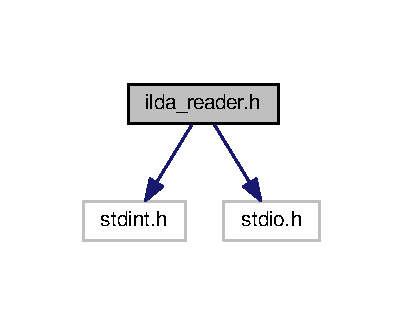
\includegraphics[width=194pt]{ilda__reader_8h__incl}
\end{center}
\end{figure}
This graph shows which files directly or indirectly include this file\+:\nopagebreak
\begin{figure}[H]
\begin{center}
\leavevmode
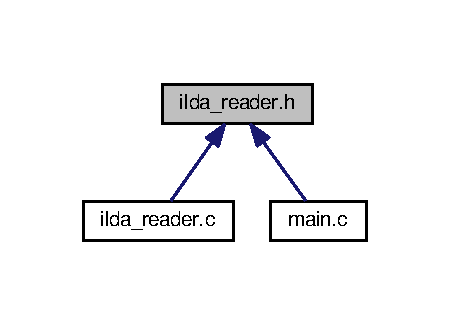
\includegraphics[width=216pt]{ilda__reader_8h__dep__incl}
\end{center}
\end{figure}
\subsubsection*{Data Structures}
\begin{DoxyCompactItemize}
\item 
struct \hyperlink{structheader__ilda}{header\+\_\+ilda}
\begin{DoxyCompactList}\small\item\em Data structure which contains the ilda header fields. \end{DoxyCompactList}\item 
struct \hyperlink{structtrue__color}{true\+\_\+color}
\begin{DoxyCompactList}\small\item\em Colour data structure for the true colour formats. \end{DoxyCompactList}\item 
struct \hyperlink{structpalette}{palette}
\begin{DoxyCompactList}\small\item\em format 2, colour palette for the formats using colour index \end{DoxyCompactList}\item 
struct \hyperlink{structpoint2__d}{point2\+\_\+d}
\begin{DoxyCompactList}\small\item\em format 1, size of 6 bytes. 2D point with colour index \end{DoxyCompactList}\item 
struct \hyperlink{structpoint3__d}{point3\+\_\+d}
\begin{DoxyCompactList}\small\item\em format 0, size of 8 bytes. 3D point with colour index \end{DoxyCompactList}\item 
struct \hyperlink{structpoint3__d__true}{point3\+\_\+d\+\_\+true}
\begin{DoxyCompactList}\small\item\em format 4, size of 10 bytes. 3D point with true colour structure. \end{DoxyCompactList}\item 
struct \hyperlink{structpoint2__d__true}{point2\+\_\+d\+\_\+true}
\begin{DoxyCompactList}\small\item\em format 5, size of 8 bytes. 2D point with true colour structure \end{DoxyCompactList}\end{DoxyCompactItemize}
\subsubsection*{Typedefs}
\begin{DoxyCompactItemize}
\item 
typedef unsigned char \hyperlink{ilda__reader_8h_a0c8186d9b9b7880309c27230bbb5e69d}{byte}
\begin{DoxyCompactList}\small\item\em byte typedef \end{DoxyCompactList}\end{DoxyCompactItemize}
\subsubsection*{Functions}
\begin{DoxyCompactItemize}
\item 
int \hyperlink{ilda__reader_8h_a658cb1acb17941afee94de570f2197b8}{read\+\_\+ilda\+\_\+header} (struct \hyperlink{structheader__ilda}{header\+\_\+ilda} $\ast$hdr, F\+I\+LE $\ast$ins)
\begin{DoxyCompactList}\small\item\em Puts ilda header information in the {\itshape hdr parameter from the ins} file. \end{DoxyCompactList}\item 
int \hyperlink{ilda__reader_8h_ad8543fa23af10e3cdbe44e62c66556a1}{read3\+\_\+dt} (struct \hyperlink{structpoint3__d__true}{point3\+\_\+d\+\_\+true} $\ast$point, F\+I\+LE $\ast$ins)
\begin{DoxyCompactList}\small\item\em Reads from a file into a \hyperlink{structpoint3__d__true}{point3\+\_\+d\+\_\+true} P\+OD structure, should be called if format code \textquotesingle{}4\textquotesingle{} is encountered. \end{DoxyCompactList}\item 
int \hyperlink{ilda__reader_8h_a42c4a3d0ee1c18a464bf952ab9e6e73d}{read2\+\_\+dt} (struct \hyperlink{structpoint2__d__true}{point2\+\_\+d\+\_\+true} $\ast$point, F\+I\+LE $\ast$ins)
\begin{DoxyCompactList}\small\item\em Reads from a file into a \hyperlink{structpoint2__d__true}{point2\+\_\+d\+\_\+true} P\+OD structure, should be called if format code \textquotesingle{}5\textquotesingle{} is encountered. \end{DoxyCompactList}\item 
int \hyperlink{ilda__reader_8h_acfc7598b101bc5f6551e0eba6079cca5}{read3\+\_\+d} (struct \hyperlink{structpoint3__d}{point3\+\_\+d} $\ast$point, F\+I\+LE $\ast$ins)
\begin{DoxyCompactList}\small\item\em Reads from a file into a \hyperlink{structpoint3__d}{point3\+\_\+d} P\+OD structure, should be called if format code \textquotesingle{}0\textquotesingle{} is encountered. \end{DoxyCompactList}\item 
int \hyperlink{ilda__reader_8h_a6ccfb058e3e717fc6b62a16975aae044}{read2\+\_\+d} (struct \hyperlink{structpoint2__d}{point2\+\_\+d} $\ast$point, F\+I\+LE $\ast$ins)
\begin{DoxyCompactList}\small\item\em Reads from a file into a \hyperlink{structpoint2__d}{point2\+\_\+d} P\+OD structure, should be called if format code \textquotesingle{}1\textquotesingle{} is encountered. \end{DoxyCompactList}\item 
int \hyperlink{ilda__reader_8h_a620cfa9600a541d1c512b0ef7a63b92b}{read\+\_\+palette} (struct \hyperlink{structpalette}{palette} $\ast$point, F\+I\+LE $\ast$ins)
\begin{DoxyCompactList}\small\item\em Reads from a file into a palette P\+OD structure, should be called if format code \textquotesingle{}2\textquotesingle{} is encountered. \end{DoxyCompactList}\item 
void \hyperlink{ilda__reader_8h_a370b6a4c6d690796ef6e62ff7b2e5f94}{read\+\_\+ilda} ()
\begin{DoxyCompactList}\small\item\em reads the whole ilda file and prints it on the console. Does not buffer anything. Will exit if file is not found. \end{DoxyCompactList}\end{DoxyCompactItemize}


\subsubsection{Typedef Documentation}
\index{ilda\+\_\+reader.\+h@{ilda\+\_\+reader.\+h}!byte@{byte}}
\index{byte@{byte}!ilda\+\_\+reader.\+h@{ilda\+\_\+reader.\+h}}
\paragraph[{\texorpdfstring{byte}{byte}}]{\setlength{\rightskip}{0pt plus 5cm}typedef unsigned char {\bf byte}}\hypertarget{ilda__reader_8h_a0c8186d9b9b7880309c27230bbb5e69d}{}\label{ilda__reader_8h_a0c8186d9b9b7880309c27230bbb5e69d}


byte typedef 



\subsubsection{Function Documentation}
\index{ilda\+\_\+reader.\+h@{ilda\+\_\+reader.\+h}!read2\+\_\+d@{read2\+\_\+d}}
\index{read2\+\_\+d@{read2\+\_\+d}!ilda\+\_\+reader.\+h@{ilda\+\_\+reader.\+h}}
\paragraph[{\texorpdfstring{read2\+\_\+d(struct point2\+\_\+d $\ast$point, F\+I\+L\+E $\ast$ins)}{read2_d(struct point2_d *point, FILE *ins)}}]{\setlength{\rightskip}{0pt plus 5cm}int read2\+\_\+d (
\begin{DoxyParamCaption}
\item[{struct {\bf point2\+\_\+d} $\ast$}]{point, }
\item[{F\+I\+LE $\ast$}]{ins}
\end{DoxyParamCaption}
)}\hypertarget{ilda__reader_8h_a6ccfb058e3e717fc6b62a16975aae044}{}\label{ilda__reader_8h_a6ccfb058e3e717fc6b62a16975aae044}


Reads from a file into a \hyperlink{structpoint2__d}{point2\+\_\+d} P\+OD structure, should be called if format code \textquotesingle{}1\textquotesingle{} is encountered. 


\begin{DoxyParams}{Parameters}
{\em point} & \hyperlink{structpoint2__d}{point2\+\_\+d} P\+OD structure to read into. Does not need to be initialized. \\
\hline
{\em ins} & File descriptor to read from. Needs to be opened in binary read mode \\
\hline
\end{DoxyParams}
\begin{DoxyReturn}{Returns}
returns -\/1 on read failure and 0 on success. 
\end{DoxyReturn}
\index{ilda\+\_\+reader.\+h@{ilda\+\_\+reader.\+h}!read2\+\_\+dt@{read2\+\_\+dt}}
\index{read2\+\_\+dt@{read2\+\_\+dt}!ilda\+\_\+reader.\+h@{ilda\+\_\+reader.\+h}}
\paragraph[{\texorpdfstring{read2\+\_\+dt(struct point2\+\_\+d\+\_\+true $\ast$point, F\+I\+L\+E $\ast$ins)}{read2_dt(struct point2_d_true *point, FILE *ins)}}]{\setlength{\rightskip}{0pt plus 5cm}int read2\+\_\+dt (
\begin{DoxyParamCaption}
\item[{struct {\bf point2\+\_\+d\+\_\+true} $\ast$}]{point, }
\item[{F\+I\+LE $\ast$}]{ins}
\end{DoxyParamCaption}
)}\hypertarget{ilda__reader_8h_a42c4a3d0ee1c18a464bf952ab9e6e73d}{}\label{ilda__reader_8h_a42c4a3d0ee1c18a464bf952ab9e6e73d}


Reads from a file into a \hyperlink{structpoint2__d__true}{point2\+\_\+d\+\_\+true} P\+OD structure, should be called if format code \textquotesingle{}5\textquotesingle{} is encountered. 


\begin{DoxyParams}{Parameters}
{\em point} & \hyperlink{structpoint2__d__true}{point2\+\_\+d\+\_\+true} P\+OD structure to read into. Does not need to be initialized. \\
\hline
{\em ins} & File descriptor to read from. Needs to be opened in binary read mode \\
\hline
\end{DoxyParams}
\begin{DoxyReturn}{Returns}
returns -\/1 on read failure and 0 on success. 
\end{DoxyReturn}
\index{ilda\+\_\+reader.\+h@{ilda\+\_\+reader.\+h}!read3\+\_\+d@{read3\+\_\+d}}
\index{read3\+\_\+d@{read3\+\_\+d}!ilda\+\_\+reader.\+h@{ilda\+\_\+reader.\+h}}
\paragraph[{\texorpdfstring{read3\+\_\+d(struct point3\+\_\+d $\ast$point, F\+I\+L\+E $\ast$ins)}{read3_d(struct point3_d *point, FILE *ins)}}]{\setlength{\rightskip}{0pt plus 5cm}int read3\+\_\+d (
\begin{DoxyParamCaption}
\item[{struct {\bf point3\+\_\+d} $\ast$}]{point, }
\item[{F\+I\+LE $\ast$}]{ins}
\end{DoxyParamCaption}
)}\hypertarget{ilda__reader_8h_acfc7598b101bc5f6551e0eba6079cca5}{}\label{ilda__reader_8h_acfc7598b101bc5f6551e0eba6079cca5}


Reads from a file into a \hyperlink{structpoint3__d}{point3\+\_\+d} P\+OD structure, should be called if format code \textquotesingle{}0\textquotesingle{} is encountered. 


\begin{DoxyParams}{Parameters}
{\em point} & \hyperlink{structpoint3__d}{point3\+\_\+d} P\+OD structure to read into. Does not need to be initialized. \\
\hline
{\em ins} & File descriptor to read from. Needs to be opened in binary read mode \\
\hline
\end{DoxyParams}
\begin{DoxyReturn}{Returns}
returns -\/1 on read failure and 0 on success. 
\end{DoxyReturn}
\index{ilda\+\_\+reader.\+h@{ilda\+\_\+reader.\+h}!read3\+\_\+dt@{read3\+\_\+dt}}
\index{read3\+\_\+dt@{read3\+\_\+dt}!ilda\+\_\+reader.\+h@{ilda\+\_\+reader.\+h}}
\paragraph[{\texorpdfstring{read3\+\_\+dt(struct point3\+\_\+d\+\_\+true $\ast$point, F\+I\+L\+E $\ast$ins)}{read3_dt(struct point3_d_true *point, FILE *ins)}}]{\setlength{\rightskip}{0pt plus 5cm}int read3\+\_\+dt (
\begin{DoxyParamCaption}
\item[{struct {\bf point3\+\_\+d\+\_\+true} $\ast$}]{point, }
\item[{F\+I\+LE $\ast$}]{ins}
\end{DoxyParamCaption}
)}\hypertarget{ilda__reader_8h_ad8543fa23af10e3cdbe44e62c66556a1}{}\label{ilda__reader_8h_ad8543fa23af10e3cdbe44e62c66556a1}


Reads from a file into a \hyperlink{structpoint3__d__true}{point3\+\_\+d\+\_\+true} P\+OD structure, should be called if format code \textquotesingle{}4\textquotesingle{} is encountered. 


\begin{DoxyParams}{Parameters}
{\em point} & \hyperlink{structpoint3__d__true}{point3\+\_\+d\+\_\+true} P\+OD structure to read into. Does not need to be initialized. \\
\hline
{\em ins} & File descriptor to read from. Needs to be opened in binary read mode \\
\hline
\end{DoxyParams}
\begin{DoxyReturn}{Returns}
returns -\/1 on read failure and 0 on success. 
\end{DoxyReturn}
\index{ilda\+\_\+reader.\+h@{ilda\+\_\+reader.\+h}!read\+\_\+ilda@{read\+\_\+ilda}}
\index{read\+\_\+ilda@{read\+\_\+ilda}!ilda\+\_\+reader.\+h@{ilda\+\_\+reader.\+h}}
\paragraph[{\texorpdfstring{read\+\_\+ilda()}{read_ilda()}}]{\setlength{\rightskip}{0pt plus 5cm}void read\+\_\+ilda (
\begin{DoxyParamCaption}
{}
\end{DoxyParamCaption}
)}\hypertarget{ilda__reader_8h_a370b6a4c6d690796ef6e62ff7b2e5f94}{}\label{ilda__reader_8h_a370b6a4c6d690796ef6e62ff7b2e5f94}


reads the whole ilda file and prints it on the console. Does not buffer anything. Will exit if file is not found. 

\index{ilda\+\_\+reader.\+h@{ilda\+\_\+reader.\+h}!read\+\_\+ilda\+\_\+header@{read\+\_\+ilda\+\_\+header}}
\index{read\+\_\+ilda\+\_\+header@{read\+\_\+ilda\+\_\+header}!ilda\+\_\+reader.\+h@{ilda\+\_\+reader.\+h}}
\paragraph[{\texorpdfstring{read\+\_\+ilda\+\_\+header(struct header\+\_\+ilda $\ast$hdr, F\+I\+L\+E $\ast$ins)}{read_ilda_header(struct header_ilda *hdr, FILE *ins)}}]{\setlength{\rightskip}{0pt plus 5cm}int read\+\_\+ilda\+\_\+header (
\begin{DoxyParamCaption}
\item[{struct {\bf header\+\_\+ilda} $\ast$}]{hdr, }
\item[{F\+I\+LE $\ast$}]{ins}
\end{DoxyParamCaption}
)}\hypertarget{ilda__reader_8h_a658cb1acb17941afee94de570f2197b8}{}\label{ilda__reader_8h_a658cb1acb17941afee94de570f2197b8}


Puts ilda header information in the {\itshape hdr parameter from the ins} file. 


\begin{DoxyParams}{Parameters}
{\em hdr} & ilda header P\+OD structure to put data in. Does not need to be initialized. \\
\hline
{\em ins} & file descriptor to read from. Needs to be opened in binary read mode. \\
\hline
\end{DoxyParams}
\begin{DoxyReturn}{Returns}
returns 0 for success, -\/1 if read failed, 1 if I\+L\+DA header is not recognized and 2 if the final header has been found. 
\end{DoxyReturn}
\index{ilda\+\_\+reader.\+h@{ilda\+\_\+reader.\+h}!read\+\_\+palette@{read\+\_\+palette}}
\index{read\+\_\+palette@{read\+\_\+palette}!ilda\+\_\+reader.\+h@{ilda\+\_\+reader.\+h}}
\paragraph[{\texorpdfstring{read\+\_\+palette(struct palette $\ast$point, F\+I\+L\+E $\ast$ins)}{read_palette(struct palette *point, FILE *ins)}}]{\setlength{\rightskip}{0pt plus 5cm}int read\+\_\+palette (
\begin{DoxyParamCaption}
\item[{struct {\bf palette} $\ast$}]{point, }
\item[{F\+I\+LE $\ast$}]{ins}
\end{DoxyParamCaption}
)}\hypertarget{ilda__reader_8h_a620cfa9600a541d1c512b0ef7a63b92b}{}\label{ilda__reader_8h_a620cfa9600a541d1c512b0ef7a63b92b}


Reads from a file into a palette P\+OD structure, should be called if format code \textquotesingle{}2\textquotesingle{} is encountered. 


\begin{DoxyParams}{Parameters}
{\em point} & palette P\+OD structure to read into. Does not need to be initialized. \\
\hline
{\em ins} & File descriptor to read from. Needs to be opened in binary read mode \\
\hline
\end{DoxyParams}
\begin{DoxyReturn}{Returns}
returns -\/1 on read failure and 0 on success. 
\end{DoxyReturn}

\hypertarget{main_8c}{}\subsection{main.\+c File Reference}
\label{main_8c}\index{main.\+c@{main.\+c}}
{\ttfamily \#include \char`\"{}ilda\+\_\+reader.\+h\char`\"{}}\\*
{\ttfamily \#include $<$stdio.\+h$>$}\\*
Include dependency graph for main.\+c\+:\nopagebreak
\begin{figure}[H]
\begin{center}
\leavevmode
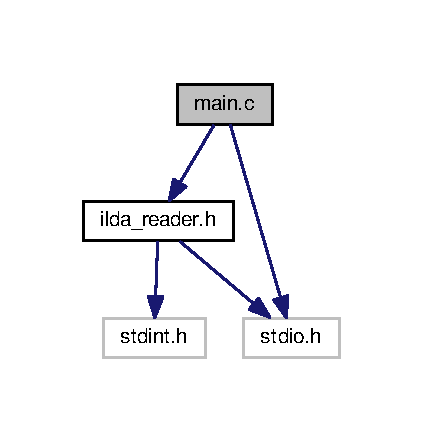
\includegraphics[width=203pt]{main_8c__incl}
\end{center}
\end{figure}
\subsubsection*{Functions}
\begin{DoxyCompactItemize}
\item 
int \hyperlink{main_8c_a0ddf1224851353fc92bfbff6f499fa97}{main} (int argc, char $\ast$argv\mbox{[}$\,$\mbox{]})
\end{DoxyCompactItemize}


\subsubsection{Function Documentation}
\index{main.\+c@{main.\+c}!main@{main}}
\index{main@{main}!main.\+c@{main.\+c}}
\paragraph[{\texorpdfstring{main(int argc, char $\ast$argv[])}{main(int argc, char *argv[])}}]{\setlength{\rightskip}{0pt plus 5cm}int main (
\begin{DoxyParamCaption}
\item[{int}]{argc, }
\item[{char $\ast$}]{argv\mbox{[}$\,$\mbox{]}}
\end{DoxyParamCaption}
)}\hypertarget{main_8c_a0ddf1224851353fc92bfbff6f499fa97}{}\label{main_8c_a0ddf1224851353fc92bfbff6f499fa97}

%--- End generated contents ---

% Index
\newpage
\phantomsection
\clearemptydoublepage
\addcontentsline{toc}{section}{Index}
\printindex

\end{document}
